\chapter{性能评估}

为了验证基于软硬协同的中断响应与任务调度设计的有效性,并且评估设计中的各个模块对系统性能的影响,本章在 FPGA 平台上围绕以下三个核心维度展开客观评价:

\begin{itemize}
    \item 任务调度:对基于 TAIC 提供的任务调度功能与传统的软件调度进行多维度对比测试,评估 TAIC 在任务窃取开销等方面的影响;
    
    \item 中断处理:评估基于 TAIC 提供的中断处理机制相较于传统中断处理机制对中断延时的影响;
    
    \item 任务通信:评估基于 TAIC 提供的任务通信能力与传统任务通信机制之间的性能差异。
\end{itemize}

\section{测试环境}

性能评估实验在 ALINX AXU15EG 开发板上展开,该开发板以 Xilinx Zynq UltraScale+ XCZU15EG MPSoC 为核心板,并配备了 DDR4、双千兆以太网接口等外部设备。核心板分为两部分,分别为处理器子系统和可编程逻辑(FPGA)。其中处理器子系统集成了四核 ARM® Cortex-A53 处理器、双核 Cortex-R5 实时处理器,可以直接对开发板上的资源进行控制。FPGA 部分实现了带有 RISC-V N 扩展的 rocket-chip 软核。rocket-chip 软核通过 TileLink 协议与 TAIC 进行交互,并且将 TileLink 协议转换成 AXI 协议来访问 DDR4 内存资源。因此,软核访问 TAIC 与内存的开销相当。

\begin{table}[htbp]
    \centering
    \caption{测试硬件环境}
    \label{tab:platform}
    \begin{tabular}{ll}
        \toprule
        \textbf{IP 核} & \textbf{配置} \\
        \midrule
        \multirow{4}{*}{RISC-V 软核} & rocket chip \\
        & 四核,N 扩展 \\
        & 100MHz 时钟 \\
        & TAIC 中断控制器 \\
        \multirow{2}{*}{以太网} & Xilinx AXI 1G/2.5G 以太网子系统(1Gbps) \\
        & Xilinx AXI DMA \\
        \bottomrule
    \end{tabular}
\end{table}

测试的硬件环境为 FPGA 平台,具体配置如表 \ref{tab:platform}。软件运行于 FPGA 中的 RISC-V 软核上,在微基准测试中,首先测试了软硬件交互接口开销,后续使用了 Linux 6.6.0 版本的基于 RISC-V 指令集的内核进行部分模块的单独测试。而综合测试基于 Rust 语言对 Sel4 \cite{sel4_2025} 重写的 Rel4 微内核 \cite{rel4_kernel} 展开,测试 TAIC 整体功能对应用程序性能的影响。

\section{微基准测试}

微基准测试主要用于从微观层面评估 TAIC 的性能表现。CPU 与 TAIC 之间的交互在几个时钟周期内完成。其中,申请硬件资源需要 4~6 个时钟周期,与任务调度相关的入队/出队操作在 2~4 个时钟周期内完成,与任务通信相关的注册(注销)发送方/接收方以及发送通知的操作在 8~10 个时钟周期内完成。TAIC 接收到中断信号把处于阻塞队列中的任务标识放入到就绪队列中的过程(中断处理),需要 6~8 个时钟周期。除软硬件交互接口测试外,其余测试在Linux 6.6.0 系统环境下完成,具体通过 tokio-bench 和 ipc-bench 两个专业工具展开。

\subsection{任务调度}

tokio \cite{tokio} 作为 Rust 生态中的高性能异步运行时框架,提供了从任务调度到 I/O 操作的全套异步工具链,用于构建高并发、低延时的网络服务。tokio 提供了 rt\_multi\_threaded 基准测试,用于评估多线程环境下的任务调度性能。tokio 的多线程调度器默认使用了任务窃取算法来动态平衡 CPU 上的任务负载,具体的规则如下:

\begin{enumerate}
    \item 针对每个工作线程,单独维护一个有界的局部队列;
    \item 所有的工作线程共用一个无界的全局队列;
    \item \label{item:push_overflow} 当局部队列达到容量上限时,任务将会被放入全局队列中;
    \item \label{item:steal_work}当局部队列没有任务时,工作线程会随机的从其他的工作线程的局部队列中窃取一半的任务;
    \item 当工作线程连续 60 次(tokio 的默认配置)从局部队列中取出任务后,将会从全局队列中取出一个任务。
\end{enumerate}

\begin{figure*}[htbp]
    \centering
    \begin{minipage}[c]{0.32\textwidth}
		\centering
		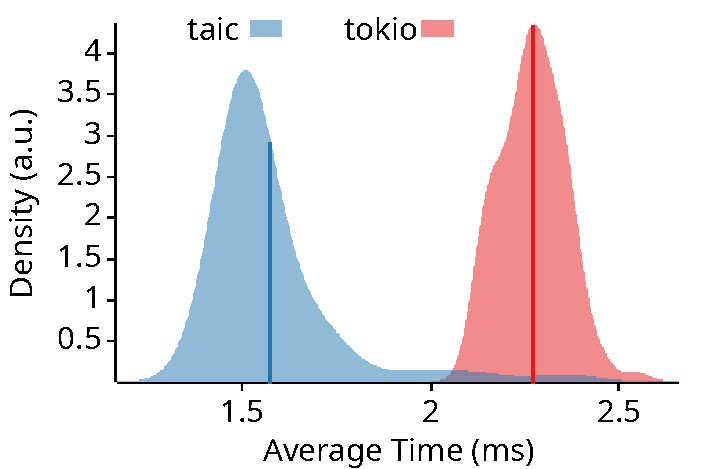
\includegraphics[width=\textwidth]{figures/tokio/chained_spawn.pdf}
		\subcaption{chained\_spawn}
		\label{tokio_chained_spawn}
	\end{minipage}
    \begin{minipage}[c]{0.32\textwidth}
		\centering
		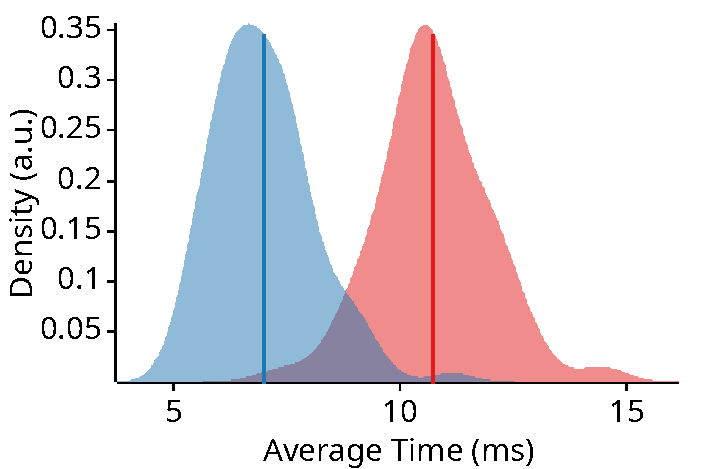
\includegraphics[width=\textwidth]{figures/tokio/spawn_local.pdf}
		\subcaption{spawn\_local}
		\label{tokio_spawn_local}
	\end{minipage}
    \begin{minipage}[c]{0.32\textwidth}
		\centering
		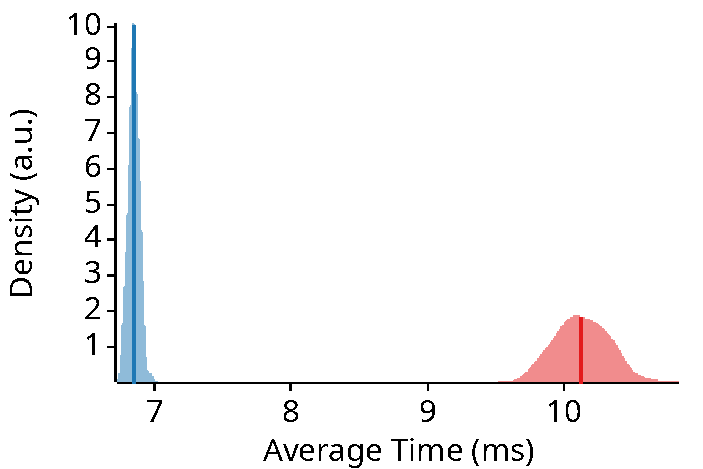
\includegraphics[width=\textwidth]{figures/tokio/spawn_remote_idle.pdf}
		\subcaption{spawn\_remote\_idle}
		\label{tokio_spawn_remote_idle}
	\end{minipage}

    \begin{minipage}[c]{0.32\textwidth}
		\centering
		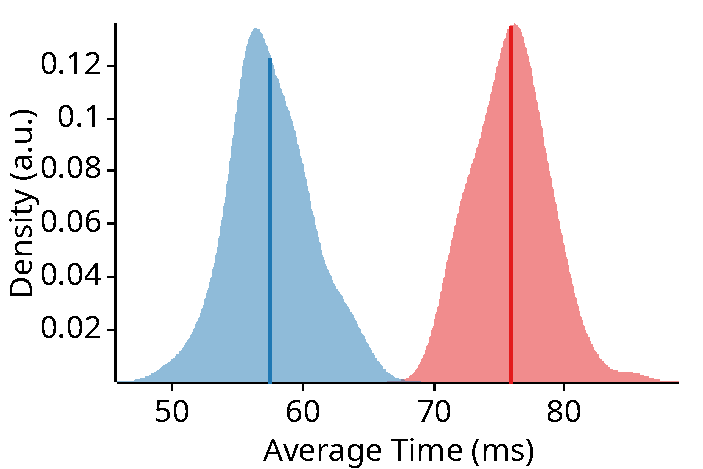
\includegraphics[width=\textwidth]{figures/tokio/yield.pdf}
		\subcaption{yield}
		\label{tokio_yield}
	\end{minipage}
    \begin{minipage}[c]{0.32\textwidth}
		\centering
		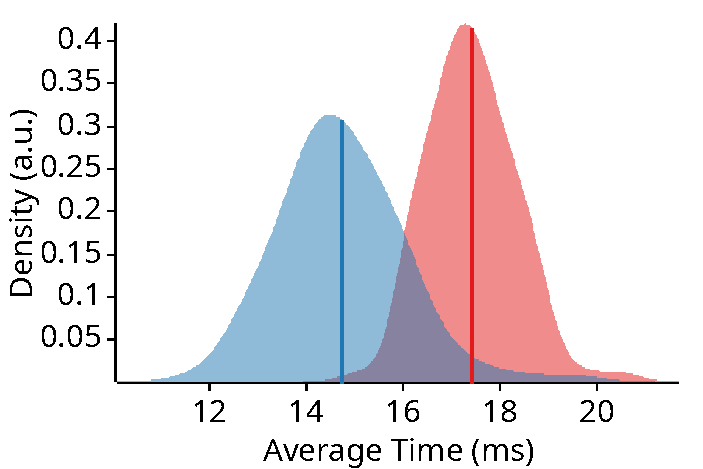
\includegraphics[width=\textwidth]{figures/tokio/ping_pong.pdf}
		\subcaption{ping\_pong}
		\label{tokio_ping_pong}
	\end{minipage}
    \begin{minipage}[c]{0.32\textwidth}
		\centering
		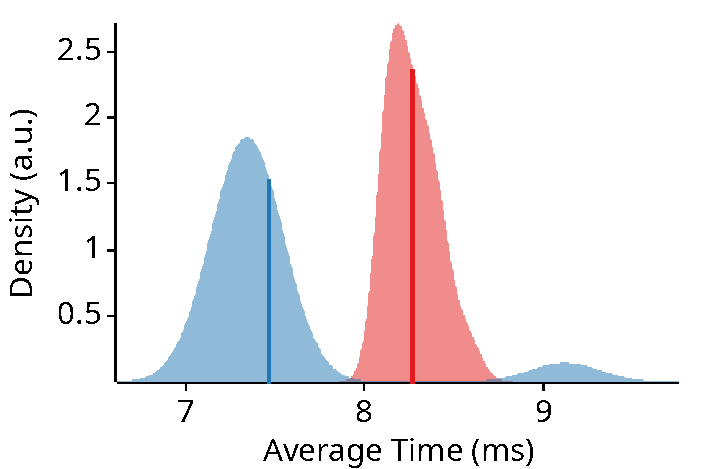
\includegraphics[width=\textwidth]{figures/tokio/spawn_remote_busy.pdf}
		\subcaption{spawn\_remote\_busy}
		\label{tokio_spawn_remote_busy}
	\end{minipage}
    \caption{任务调度对比,其中 taic 表示使用硬件任务队列,tokio 表示使用软件任务队列。}
    \label{figure:tokio-bench}
\end{figure*}

本文对 tokio 默认的多线程调度器进行了修改,将其任务窃取算法中使用的任务队列替换为 TAIC 提供的硬件任务队列。每个工作线程使用 TAIC 提供的硬件局部队列,这些硬件局部队列共同构成一个硬件全局队列,如图 \ref{figure:ready_queue} 所示。由于硬件的局部队列没有固定的容量限制,但其最大容量不超过全局队列的容量,因此修改后的 tokio 任务调度器无法满足规则 \ref{item:push_overflow},为了保证公平,测试过程中保证了不会出现局部队列溢出的情况。此外,由于硬件提供了局部队列之间的负载均衡功能,当局部队列中没有任务时,会自动从其他的局部队列中取出任务,因此,规则 \ref{item:steal_work} 也不再需要,但保留了计算随机数的开销来保证测试的公平性。使用上述修改后的 tokio 调度器来评估 TAIC 在任务调度方面的性能表现,最终的结果如图\ref{figure:tokio-bench}所示。

\textbf{任务窃取}:chained\_spawn 测试递归的生成任务,任意时刻,至多存在两个任务,当一个工作线程运行任务 $A$ 生成一个新的任务 $B$ 时,其他的空闲的工作线程会窃取新生成的任务 $B$ 来执行,循环这个过程,直到结束。因此两个测试的性能差异主要取决于任务窃取的性能。taic 在任务窃取时直接从局部队列中可以窃取出其他的局部队列中的任务,而 tokio 原本的软件任务窃取需要搜索开销以及局部队列的同步互斥等额外开销,从图 \ref{tokio_chained_spawn} 可以看出,taic 使得任务窃取的开销下降了 30.68\%。同理,spawn\_local 测试生成更多的任务,并将任务放入当前工作线程的局部队列中,尽管 tokio 原本的任务窃取会直接从其他局部队列中窃取一半的任务,但 taic 提供的硬件任务窃取功能几乎是零开销的,因此,taic 在 spawn\_local 测试(图\ref{tokio_spawn_local})中仍然将任务窃取的开销下降了 34.88\%。spawn\_remote\_idle 测试(图\ref{tokio_spawn_remote_idle})与 spawn\_local 测试类似,不同之处在于它将生成的任务放到了远端队列(远端队列等价于局部队列,用于任务窃取)中,两者的性能差距仍然来源于任务窃取的开销(32.41\%)。

\textbf{任务切换}:yield(图 \ref{tokio_yield})、ping\_pong(图 \ref{tokio_ping_pong}) 和 spawn\_remote\_busy(图 \ref{tokio_spawn_remote_busy}) 测试了在高频任务切换时,硬件任务队列与软件任务队列的性能差异。在 yield 测试中,每个任务在主动让权若干次后结束;在 ping\_pong 测试中,由于相互发送消息的两个任务需要等待对方的消息;在spawn\_remote\_busy 测试中,用户态任务让权后再次运行时,会使用 \verb|sched_yield| 系统调用让当前的工作线程进入内核态让权。因此,使用 taic 节省的任务窃取开销被分摊到每次任务切换以及等待的过程中,使用 taic 将这三个测试的开销分别降低了 24.22\%、15.37\% 和 9.69\%。其中 spawn\_remote\_busy 测试过程中,因为 Linux 内核产生随机数缓慢,导致了使用 taic 时部分测试的平均延时过高。

\subsection{任务通信}

ipc-bench \cite{ipc-bench_2025} 是一个用于测试 Linux 上的包括信号、管道和 eventfd 等 IPC 机制的开源项目。ipc-bench 针对每种 IPC 机制使用了 ping-pong 通信模型(通信双方忙等对方的消息)来测试其性能,性能指标包括通行的总时间、平均每次通信的时间、吞吐量等。

本文参考 ipc-bench 项目中对信号、管道和 eventfd 等 IPC 机制的测试方法,实现了使用 TAIC 进行任务通信的测试程序。测试程序排除了申请 TAIC 硬件资源以及初始化的时间,测试了通信的总时间。其中,所有测试的消息大小为 1 bit,发送消息次数为 1000 次。各项 IPC 机制的性能对比如图 \ref{figure:ipc-bench} 和表 \ref{tab:ipc-bench} 所示。

\begin{figure}
    \centering
    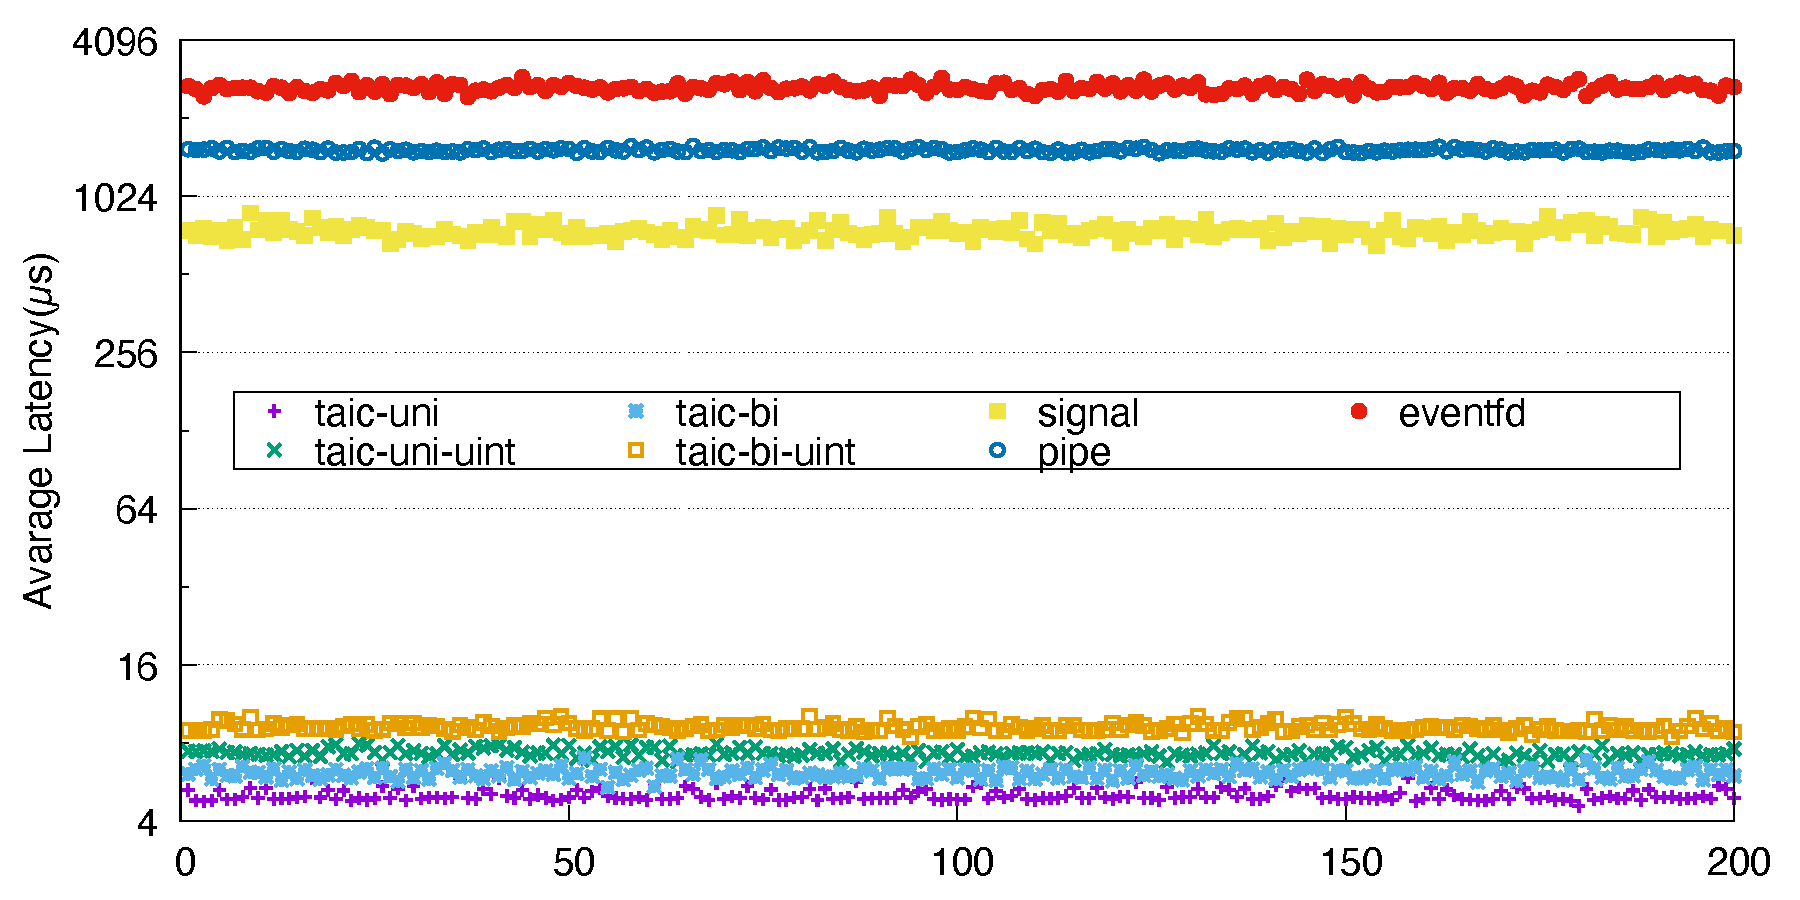
\includegraphics[width=\textwidth]{figures/pdfs/taic-ipc.pdf}
    \caption{IPC 延迟对比,taic 表示使用硬件任务通信机制的测试。其中,bi 表示双向,双方互相发送消息;uni 表示单向;uint 表示任务优先级高,需要发送中断。eventfd、pipe、signal 均为双向;}
    \label{figure:ipc-bench}
\end{figure}

\begin{table}
    \centering
    \caption{IPC 性能对比}
    \label{tab:ipc-bench}
    \begin{tabular}{llll}
        \toprule
        \textbf{测试} & \textbf{吞吐量 $msg/s$} & \textbf{平均延时 $\mu s$} & \textbf{相对延迟比} \\
        \midrule
        taic-uni & 199215.0 & 5.02 & 1 \\
        taic-bi & 163158.4 & 6.13 & 1.221 \\
        taic-uni-uint & 137127.0 & 7.29 & 1.453 \\
        taic-bi-uint & 108734.7 & 9.20 & 1.832 \\
        signal & 1334.7 & 749.23 & 149.258 \\
        pipe & 649.6 & 1539.41 & 306.673 \\
        eventfd & 374.9 & 2667.38 & 531.382 \\
        \bottomrule
    \end{tabular}
\end{table}

与 taic 相关的测试保证了通信的接收方在 CPU 上运行(接收方处于在线状态)。不使用中断时,接收方不断尝试从硬件任务队列中取出被唤醒的任务,一旦取出任务则表示收到通知,结束通信的过程;当使用中断时,接收方收到中断信号后,进入用户态的中断的处理逻辑中,从硬件任务队列中取出被唤醒的任务才算收到通知,但需要从中断返回才结束通信;在双向通信中,接收方收到发送方的通知后,向发送方发起通知,直到发送方收到通知才结束通信的流程。

无论是否使用中断来进行任务抢占,使用 TAIC 进行任务通信的性能都远远优于其他的 IPC 机制,在性能上有数量级的提升,能够达到微秒级的时间尺度。但在不使用中断的情况下,若接收方进程正在执行其他的任务,TAIC 内部的中断处理和中断的开销会被其他任务执行掩盖掉,若其他任务的执行时间也处于微秒级,那么即使不需要中断机制,同样可以达到微秒级的通信延迟。

在 ipc-bench 测试的基础上,本文进一步测试了接收方处于不同的特权级的中断延迟(中断延迟包括了 TAIC 中断处理开销、保存被打断任务上下文开销以及软件进行中断分发的开销)。具体的结果如表 \ref{tab:interrupt-latency}所示,括号内表示不包括 TAIC 中断处理开销的中断延迟。结果证明了使用 TAIC 不会增加中断延迟,保证被唤醒的任务可以及时抢占。

\begin{table}
    \centering
    \caption{中断延迟对比}
    \label{tab:interrupt-latency}
    \begin{tabular}{ll}
        \toprule
        \textbf{接收方特权级} & \textbf{CPU 周期} \\
        \midrule
        用户态 & 72(66) \\
        内核态 & 98(92) \\
        \bottomrule
    \end{tabular}
\end{table}

以上的测试没有包括极端的情况。一种极端的情况是接收方运行于用户态,但接收方的进程没有任务在用户态运行,此时,即使唤醒的任务的优先级较高,也无法进行任务抢占,需要等到接收方的进程中存在任务回到用户态运行时才能进行抢占,此时,任务通信的延时除了用户态中断的开销外,还包括了接收方进程等待被调度的时间以及从内核态返回用户态的开销。另一种极端的情况是接收方运行于内核态,但此时接收方没有任务处于内核态运行,因此任务抢占会导致一个正在运行用户态任务的 CPU 陷入内核态,因此任务通信的开销还会包括特权级切换开销(在本文的实验环境下,开销为 870 个时钟周期)。

\section{综合测试}

\subsection{特征分析}

\section{本章小结}

% 从硬件出发的角度,大多数工作通过设计特殊的硬件或者特殊的指令来绕过内核实现 IPC。如 SkyBridge[11]允许进程在 IPC 中直接切换到目标进程的虚拟地址空间并调用目标函数,它通过精心设计一个虚拟化层(Root Kernel)提供虚拟化的功能,通过 VMFUNC 地址空间的直接切换,并通过其他一系列软件手段来保证安全性,但这种方案仅适用于虚拟化环境中。XPC[12]则直接使用硬件来提供一个无需经过内核的同步功能调用,并提供一种新的空间映射机制用于调用者与被调用者之间的零拷贝消息传递,然而该方案没有相应的硬件标准,也没有一款通用的处理器对其进行支持。这些方法都基于特殊的环境或者没有标准化的硬件来实现,适用范围有限。

% 从软件出发的角度,相关工作主要分为两类:第一类方法通过将用户态和内核态的功能扁平化来减少内核与用户态的切换开销,如 unikernel[13, 14, 15]将所有用户态代码都映射到内核态执行,Userspace Bypass[16]通过动态二进制分析将两个系统调用之间的用户态代码移入内核态执行,从而减少陷入内核的次数,kernel bypass[17, 18]则通过将硬件驱动(传统内核的功能)移入用户态,从而减少上下文的切换。这些方法要么需要特殊的硬件支持,要么难以与微内核的设计理念兼容。第二类方法则是允许用户空间对多个系统调用请求排队,并通过一次提交将他们注册给内核,如 FlexSC[19]通过在用户态设计一个用户态线程的运行时,将用户态线程发起的系统调用自动收集,然后陷入内核态进行批量执行。该方法虽然可以有效的减少陷入内核的次数,但如何设置提交的时机难以把握,过短的提交间隔将导致切换次数增加,过长的提交间隔则会导致 CPU 空转。

% 虽然现有工作难以广泛且有效地应用到微内核中,但他们的思路值得我们借鉴,他们的缺陷驱使我们去寻求更好的方案。在硬件方面,一种新型的硬件技术方案——用户态中断[20, 21]逐渐被各个硬件平台(x86,RISC-V)采纳,它通过在 CPU 中新增中断代理机制和用户态中断的状态寄存器,当中断代理机制检测到状态寄存器发生变化时,会将中断以硬件转发的形式传递给用户态程序,从而绕过内核。该硬件方案已经在 Sapphire Rapids x86 处理器上和 RISCV 的 N 扩展中有了一定的支持,适用范围更加广泛。而在软件方面,异步被广泛用于请求合并和开销均摊,传统类 Unix 系统提供的类似 select IO 多路复用接口相对简陋,迫使用户态代码采用事件分发的编程范式来处理异步事件,代码相对复杂,可读性较弱。而新兴的 Rust[22, 23]语言对异步有着良好的支持,其零成本抽象的设计也让它作为系统编程语言有着强大的竞争力。使用 Rust 进行内核和用户态基础库的开发,可以更好地对异步接口进行抽象,改善接口的易用性和代码的可读性。

% 我们在FPGA平台上对TAIC进行了一系列评估,旨在解决几个核心问题:

% 上下文切换的影响:我们首先评估了TAIC的快速唤醒机制相对于传统中断机制的性能优势,以了解其性能益处的来源。

% CPU利用率的影响:其次,我们检查了TAIC的快速唤醒机制对CPU利用率的影响。理解这一点对于评估TAIC在提高CPU利用率和降低CPU负载方面的有效性至关重要。

% 优先队列对I/O请求处理的影响:我们还研究了TAIC内部的优先队列如何影响不同优先级的I/O请求处理。这有助于我们理解TAIC在处理复杂I/O工作负载时的性能特点。

% 实际应用中的性能改进:最后,我们探讨了TAIC在实际应用场景中提供的延迟和吞吐量的改进程度。这项评估将为我们提供TAIC在现实条件下的性能数据,使我们能够评估其对整体系统性能的贡献。

% 通过这些评估,我们希望全面了解TAIC的性能特点,并为未来的优化和应用提供实证基础。

% 实验设置

% 为了评估TAIC的性能,我们选择了Xilinx的Zynq UltraScale+ XCZU15EG-2FFVB1156 MPSoC作为我们的FPGA平台。这款高性能的系统级芯片(SoC)为我们提供了充足的资源来实现复杂的硬件加速任务。我们的工作基于Rocket-chip项目[3],这是一个开源的RISC-V架构,五级流水线处理器软核(四核,100MHz)。利用这个基础,我们实现了TAIC中断控制器,以利用其快速唤醒功能机制。此外,我们构建了一个高效的异步网络卡驱动程序,专门设计用于处理网络I/O请求。我们选择了Xilinx AXI 1G/2.5G以太网子系统(1Gbps)作为我们的网络接口,并配备了Xilinx AXI DMA控制器以促进高速数据传输。

% 异步 IPC 作为 ReL4 中的主要的 IPC 方式,其实现依赖于异步运行时和 U-notification。我们以 IPC 中最常见的 Call为例,客户端进程和服务端进程在双方建立连接时都会注册一个 dispatcher 协程用于不断从共享缓冲区中读取数据并进行处理。我们分别对服务端和客户端的 dispatcher 协程提供了两个默认实现,对于特殊的需求,用户程序可以通过运行时接口自定义 dispatcher 协程的行为。服务端的 dispatcher协程读取请求并处理后将响应写入环形缓冲区,并根据标志位判断是否发送 U-notification,没有请求时阻塞自己并切换到其他 worker 协程。客户端的 dispatcher 协程读取响应并唤醒响应的协程,没有响应时阻塞切换。Call 的主要流程分为以下几个阶段:

% 1)客户端发起请求:用户态程序将以 worker 协程的形式发起 IPC 请求,异步运行时首先会根据请求的数据和协程的协程号生成 IPCItem 并写入请求的环形缓冲区中并将当前协程阻塞,然后检查缓冲区的 req\_co\_status 标志位,如果对方的 dispatcher 协程已经就绪,那我们无需通知对方进程,对方进程的异步运行时会在某个时刻调度到 dispatcher协程并处理请求。如果对方的 dispatcher 协程处于阻塞状态,则异步运行时会将 req\_co\_status 标志位置位,并发送 Unotification 通知对方进程唤醒 dispatcher 协程并重启调度。

% 2)服务端处理请求并写回响应:服务端的 dispatcher 协程会在合适的时机读取出请求并进行解码和处理,然后根据处理结果构造响应的 IPCItem 并写入响应的环形缓冲区中,检查缓冲区中的 reply\_co\_status 标志位,如果客户端的响应 dispatcher 协程就绪,则无需发起通知,否则需要发起 Unotification 通知客户端进程唤醒 dispatcher 协程并重启调度。如果缓冲区内容为空,dispatcher 协程会将 req\_co\_status 标志位置空,并将自己阻塞。

% 3)客户端处理响应:客户端的 dispatcher 协程会在合适的时机读取响应并唤醒之前阻塞的协程,然后重启调度。

% 从广义的角度来看,异步系统调用是一类特殊的异步IPC,其接收方为内核。因此我们在内核中提供了一套相似的异步运行时以支持异步系统调用。异步系统调用与异步IPC 的主要不同之处有两点:

% 1) 由于接收端是内核,发送端无法使用 U-notification 去通知内核。

% 2) 异步 IPC 中进程的异步调度器就是进程的执行主体,无需考虑异步任务的执行时机,而内核除了异步系统调用请求需要调度器执行,本身就有如中断、异常、任务调度等其他任务需要被执行。对于第一点,我们只需要新增一个系统调用去用于唤醒相关的内核协程即可。而对于第二点,一个很简单的思路是每次时钟中断到来时去执行异步系统调用,然而这可能会导致空闲的 CPU 核心无法及时触发时钟中断而空转,因此,在不破坏原本的线程优先级调度前提下,我们使用核间中断来抢占空闲 CPU 核心或正在运行低优先级线程的 CPU 核心,更好地利用空闲 CPU 资源,减少响应时延。为了避免破坏微内核中原本的优先级调度机制,我们在内核中对 每 个 CPU 核心维护了相应的执行优先级(exec\_prio),执行优先级区别于上文提到的运行时协程优先级,是由内核调度器维护的线程优先级。内核中的任务主要分为三类:1) idle\_thread: 空闲 CPU 核心执行 idle 线程,此时 CPU 核心的执行优先级为 256,属于最低的执行优先级。2) 内核态任务:正在处理中断、异常、系统调用等,此时CPU 核心的执行优先级为 0,最高优先级,不可被抢占。3) 用户态任务:正在执行用户态的任务,此时 CPU 核心的执行优先级为当前线程的优先级,可以被更高优先级线程提交的异步系统调用请求打断。

% 当发送端通过系统调用陷入内核去唤醒相应协程后,会检查当前线程的优先级是否可以抢占其他 CPU 核心,如果可以,则发送核间中断抢占该 CPU 核心去执行异步系统调用,当前 CPU 核心则返回用户态继续执行其他协程。如果没有可以被抢占的 CPU 核心,则在下一次时钟中断到来时执行异步系统调用请求,其伪代码如下:

% 为了从微观角度评估我们设计的异步 IPC 性能,我们测量了不同并发量和不同服务端负载下异步 IPC 和同步 IPC的平均开销。由于我们关注的是同步 IPC 和异步 IPC 的路径差异,需要保证场景没有过多干扰,因此我们分别构建了一个服务端进程和一个客户端进程进行乒乓测试,测试结果如图 5 所示。

% 由于同步 IPC 会阻塞整个线程,因此并发量对同步 IPC并没有意义。而在多核环境下,fast-path 检查会失败,所有的同步 IPC 都会在内核中通过核间中断进行传递,因此多核环境下的同步 IPC 性能很低;而对于单核下的同步 IPC,fast-path 会避开复杂的消息解码和冗长的调度流程,因此开启fast-path的IPC性能会提升167\%,但我们需要注意的是,fast-path 对于线程优先级、消息长度等有着严苛的检查流程,因此在实际应用场景中 fast-path 优化并不总能生效。

% 我们从横向的角度分析异步 IPC,发现异步 IPC 的开销随着并发量的提升而降低,这是由于随着并发量的增加,服务端的负载进一步增加,而 U-notification 的通知时机采用自适应的形式,因此通知频率下降,导致了均摊到每个 IPC的开销下降。我们还可以看出,在并发度较小的时候,多核会略快于单核(最高提升 52\%),符合预期,随着并发度的逐渐增加,多核与单核的性能差异逐渐缩小(17\%),这是由于多核情况下服务端单独使用一个 CPU 核心,导致服务端负载过小,产生了更加频繁的用户态中断(如左图中的蓝色折线),导致服务端吞吐量过小,又反过来限制了客户端的请求频率。可以从第二幅图中看出,当我们增加服务端负载时,服务端的中断频率会逐渐下降,直至归 0,这是自适应轮询带来的优势。

% 对比同步 IPC 和异步 IPC,当并发度为 1 的时候,每个异步 IPC 的开销都包含了两次用户态中断的开销、调度器的运行时开销,而同步 IPC 则是两次特权级切换的开销,如果没有 fast-path 优化,还会有内核路径中的解码开销和调度开销,因此在低并发度的场景下异步 IPC 的性能会略低于没有fast-path 优化的同步 IPC(31\%),同时显著低于有 fast-path优化的同步 IPC(249\%)。而当并发量较大时,用户态中断的频率减少,均摊到每一次 IPC 下,用户态中断的开销几乎可以忽略不计,因此异步 IPC 的开销主要是调度器的运行时开销,而此时的异步 IPC 性能会显著高于没有 fast-path 优化的同步 IPC(369\%),也高于有 fast-path 优化的同步 IPC(76\%)。

% 从上面我们可以得出结论:在多核场景下,我们的异步IPC 相比于同步始终有着良好的表现。而在单核且低并发度场景下,异步 IPC 性能会比较差,但随着并发度增加,异步IPC 的性能会迅速提升,在并发度为 2 时就已经超过没有fast-path 优化的同步 IPC,在并发度为 8 时就已经超过了开启 fast-path 优化的同步 IPC,因此异步 IPC 依然十分有竞争力。

% 为了测试异步 IPC 在真实应用场景带来的收益,我们在ReL4 上实现了一个 TCP 服务器。模拟的 TCP 服务器应用场景由三部分组成,一部分是运行在 PC 上的客户端,它在启动时与运行在 FPGA 上的 TCP Server 建立若干个连接,并不断地向服务端发送 64 字节(小包)的数据,并接收服务器的响应;第二部分是运行在 ReL4 上的网络协议栈服务器(NW Stack Server),集成了网卡驱动的代码,并通过smoltcp 协议栈维护每个连接的状态信息,负责从网卡中接收数据并进行协议处理后通过共享缓冲区返回给 TCP Server,以及从 TCP Server 接收数据并通过网卡发出;第三部分是 TCP Server,它以 IPC 的形式从 NW Stack Server 接收客户端发送过来的请求,在处理完成之后返回响应并通过NW Stack Server 发送给客户端。最后,PC 上的客户端计算发送每个请求和接收响应之间的时间延迟,并计算固定时间段内的消息吞吐量。我们通过分析不同配置下 TCP Server 的时间延迟和吞吐量来评估 ReL4。需要注意的是,由于同步 IPC 的无法支持多路复用,因此同步 IPC 下每个连接都使用单独的线程来监听。测试结果如图 6 所示。

% 从总体趋势上看,吞吐量随着并发度的增加呈现先增加后减少的趋势,而时延成整体上升的趋势。在低并发度条件下的系统负载处于较低水平,随着并发度增加,吞吐量能稳步提升,随着系统满载之后,继续增加并发度,会导致网络中断频率上升,从而限制系统的整体性能,吞吐量减少。

% 同步和异步对比来看,可以看出当连接数较低,并发度较小的情况下,异步 IPC 实现的 TCP Server 无论是在吞吐率还是平均时延上都要优于同步 IPC,这是由于同步 IPC 需要频繁陷入内核,而由于微内核不可被抢占的设计,内核态屏蔽了网络中断,导致网络包无法及时处理。而随着并发度的增加,由于同步 IPC 实现的 TCP Server 需要多线程来保证多连接,因此线程切换的开销急剧加大,导致同步和异步的差距进一步增加。在连接数为 4 的时候差距达到最大,为192\%,在并发度最大的情况下,异步 IPC 实现的 TCP Server也比同步 IPC 高出 120\%。

% 单核与多核对比来看,异步 IPC 实现的 TCP Server 随着 CPU 资源增加,吞吐量提升,时延降低,而对于同步 IPC实现的 TCP Server 情况则有所不同,由于同步 IPC 在多核下采用的 IPI 的形式在内核进行转发,导致程序的内存局部性和代码局部性都不够友好,因此多核的性能变现会略低于单核。

% 从上面我们可以得出结论:异步 IPC 在实际应用场景中有利于多路复用的实现,可以有效减少特权级切换的开销,提升系统的整体性能。
